% 论文复现报告：Calibrate Before Use（G17 / P33）
% 编译：xelatex report.tex（两遍）
\documentclass[11pt,a4paper]{ctexart}
\usepackage[margin=2.5cm]{geometry}
\usepackage{graphicx}
\usepackage{booktabs}
\usepackage{multirow}
\usepackage{xcolor}
\usepackage{caption}
\usepackage{amsmath}
\usepackage[hidelinks]{hyperref}
\captionsetup{font=small}
\setlength{\parskip}{2pt}

\begin{document}
\begin{center}
{\LARGE\bfseries 论文复现报告：Calibrate Before Use}\\[4pt]
{\large 组号 G17 \quad 论文号 P33}\\[2pt]
{\small 复现论文：T. Zhao, E. Wallace, S. Feng, D. Klein, S. Singh.
\emph{Calibrate Before Use: Improving Few-Shot Performance of Language Models}. ICML 2021.}
\end{center}

\section{原文定位与复现范围}

原文的核心声称是：语言模型做 few-shot 分类时，对各类别的答案先验（在内容无关输入下依然存在）
会导致预测系统性偏移（miscalibration）；用内容无关输入探测该先验 $p_{\mathrm{cf}}$ 并做线性校准，
可以提升准确率并降低方差。本组按提交约定做\textbf{缩规模部分复现}，对应原文三处结论：

\begin{itemize}\itemsep1pt
  \item \textbf{Table 4（附录 A，主目标）}：GPT-2 XL（1.5B）在 SST-2 / AGNews / TREC 上的
        0/1/4/8-shot 分类，校准提升准确率并降方差；
  \item \textbf{Figure 1（GPT-2 部分）}：准确率均值与方差随 shot 数的变化，基线 vs 校准；
  \item \textbf{Table 3（附录 A）}：内容无关输入的选择（N/A、[MASK]、空串、三者平均）影响结果，
        且存在多种好选择。
\end{itemize}

与原文的差异范围：模型从 GPT-3 API（175B/13B/2.7B）换为\textbf{本地 GPT-2 四规格}
（124M / 355M / 774M / 1.5B，主实验 gpt2-xl 对应 Table 4，其余三档为本组自扩的缩规模扫描）；
任务只做原文三类任务中的\textbf{文本分类}（SST-2 二类、AGNews 四类、TREC 六类），
不做 LAMA 与抽取任务。

\section{方法与基线}

\textbf{基线（greedy）}：与作者代码一致的 prompt 格式（前缀 + few-shot 训练样例 +
``Q: \{输入\} A:''），对每个类别的标签词取首 token 概率（top-$k{=}100$；
top-$k$ 未覆盖的标签词用回声模式精确补全），归一化后取 $\arg\max$ 作为预测。

\textbf{上下文校准}：用三个内容无关输入（\texttt{N/A}、空串、\texttt{[MASK]}）分别替换测试输入，
得到模型的答案分布并取平均、归一化为先验 $p_{\mathrm{cf}}$；令
\begin{equation}
  W = \operatorname{diag}(p_{\mathrm{cf}})^{-1}, \qquad b = 0, \qquad
  \hat y = \arg\max\,(W\,\hat p + b),
\end{equation}
其中 $\hat p$ 为测试样本的归一化标签概率。直觉是：若模型对某类有 $p_{\mathrm{cf}}^{(i)}$ 的先验
偏好，则用 $1/p_{\mathrm{cf}}^{(i)}$ 加权抵消它。

\section{与原文及作者代码的设置差异}

\begin{table}[h]\centering\small
\begin{tabular}{p{3.1cm}p{4.6cm}p{6.6cm}}
\toprule
\textbf{项} & \textbf{原文 / 作者代码} & \textbf{本组设置与影响} \\
\midrule
模型 & GPT-3 API（175B/13B/2.7B）；作者代码支持本地 GPT-2 & 本地 GPT-2 四规格，fp32；
主实验 gpt2-xl 直接对应 Table 4 \\
评估规模 & 论文为更大评估集 & 每数据集固定 300 条测试子集（seed 0 冻结，跨 seed 复用），
规范允许固定子集；样本 ID 见逐条结果 \\
SST-2 测试集 & 作者仓库缺失该文件 & 取公开镜像 \texttt{stsa.binary.test}（1821 条），
同为 Socher SST 标准划分 \\
标签概率缺失 & 作者默认 \texttt{-{}-approx} 置零近似 & 总是回声补全（精确计算），
对应作者 \texttt{all\_found} 口径 \\
实现 & 作者仓库 \texttt{few-shot-learning} master（2026-11-03 读取） &
本组重实现并逐行对齐 prompt 前后缀、标签词、抽样与校准逻辑；共 9 项差异逐条声明于
\texttt{code/README.md} \S6 \\
随机性 & 多个训练样例集合 & 每配置 5 个训练样例集合（seed 0--4），prompt 格式固定为附录 B 主格式 \\
AI 辅助 & --- & 工程实现与批量执行使用 Claude Code 辅助（详见附录 A）；
方案设计、结果判读与结论由本组完成 \\
\bottomrule
\end{tabular}
\caption{与原文及作者代码的主要设置差异。}
\end{table}

\section{实验设置}

全部实验为\textbf{本机真实运行}：$4\ (\text{模型}) \times 3\ (\text{数据集}) \times 4\ (\text{shots})
\times 5\ (\text{seeds}) = 240$ 个 run，fp32 推理，无一失败；环境为 Python 3.11 +
torch 2.14.1+cu126 + transformers 5.22.1，单卡 RTX 4060 Laptop 8GB。
批处理大小按（模型 $\times$ 数据集）显存探针核定（表~\ref{tab:bs}）；
gpt2-xl fp32 权重约 6.0 GiB（文件 6.43 GB），推理峰值预留最高 8.16 GB，超出
8GB 物理显存的部分由 Windows WDDM 共享内存溢出兜底，
实测 bs=2 反而最快（溢出页少），全程无 OOM 崩溃。全网格总耗时 1 小时 40 分
（gpt2 6.6 min / medium 13.5 min / large 27.2 min / xl 52.5 min）。

\begin{table}[h]\centering\small
\begin{tabular}{lccc}
\toprule
bs（sst2 / agnews / trec） & gpt2 & gpt2-medium & gpt2-large \quad / \quad gpt2-xl \\
\midrule
峰值显存（GB） & 4.32 / 5.44 / 2.42 & 5.92 / 5.46 / 3.76 & 6.47 / 5.89 / 5.35 \quad / \quad 7.04 / 8.16 / 6.65 \\
采用 bs & 16 / 16 / 16 & 16 / 8 / 16 & 12 / 4 / 12 \quad / \quad 2 / 2 / 2 \\
\bottomrule
\end{tabular}
\caption{批处理大小核定（8-shot 最长 prompt 探针，含全池最长样本）。}
\label{tab:bs}
\end{table}

运行证据：\texttt{results/summary.csv}（240 行）、\texttt{results/logs/}（批次日志）、
\texttt{results/raw/}（每次运行的完整配置与训练样例 ID）、\texttt{results/samples/}（逐样本 CSV）；
\texttt{scripts/check\_results.py} 对全部 241 个结果文件做独立复算（从逐样本概率重算准确率、
翻转数并与 summary 交叉核对），全部通过。

\section{主要结果}

\begin{table}[h]\centering\small
\begin{tabular}{lccc}
\toprule
0-shot（基线 $\rightarrow$ 校准） & SST-2 & AGNews & TREC \\
\midrule
gpt2 (124M)        & 0.7267 $\rightarrow$ 0.6067 (\textcolor{red}{$-$12.0}) & 0.5900 $\rightarrow$ 0.5400 (\textcolor{red}{$-$5.0}) & 0.2600 $\rightarrow$ 0.1167 (\textcolor{red}{$-$14.3}) \\
gpt2-medium (355M) & 0.5933 $\rightarrow$ 0.7667 (\textcolor{blue}{$+$17.3}) & 0.3033 $\rightarrow$ 0.5333 (\textcolor{blue}{$+$23.0}) & 0.2733 $\rightarrow$ 0.0267 (\textcolor{red}{$-$24.7}) \\
gpt2-large (774M)  & 0.7167 $\rightarrow$ 0.8500 (\textcolor{blue}{$+$13.3}) & 0.3667 $\rightarrow$ 0.5333 (\textcolor{blue}{$+$16.7}) & 0.3400 $\rightarrow$ 0.1533 (\textcolor{red}{$-$18.7}) \\
gpt2-xl (1.5B)     & 0.5667 $\rightarrow$ 0.7267 (\textcolor{blue}{$+$16.0}) & 0.4100 $\rightarrow$ 0.5200 (\textcolor{blue}{$+$11.0}) & 0.2867 $\rightarrow$ 0.2100 (\textcolor{red}{$-$7.7}) \\
\bottomrule
\end{tabular}
\caption{0-shot 基线 vs 校准准确率（括号内为百分点变化；0-shot 无训练样例，无 seed 方差）。}
\label{tab:zeroshot}
\end{table}

\textbf{结论一（复现成功）：校准收益呈规模依赖。}0-shot 校准在 Medium/Large/XL 上
SST-2（$+$13--17pp）与 AGNews（$+$11--23pp）全面正收益，而 124M 的 gpt2 反向
（表~\ref{tab:zeroshot}）。这与我们中期基于 12 个冒烟 run 提出的"规模依赖"假设一致：
信号弱的模型上 $1/p_{\mathrm{cf}}$ 加权会放大噪声。原文 Figure 1 与 Table 4 的主结论
（校准提升平均准确率）在 $\geq$355M 规模上方向复现。

\textbf{结论二（与原文不一致）：TREC 上校准全面有害，且全规模成立。}原文 Table 4 中
GPT-2 XL 在 TREC 全部 shot 校准均大幅正收益（如 0-shot 24.0$\rightarrow$37.3，
1-shot 21.5$\rightarrow$41.1）；本组 gpt2-xl 的 TREC 则\textbf{全部为负}
（0-shot $-$7.7、1-shot 0.2707$\rightarrow$0.0320、8-shot 0.3753$\rightarrow$0.2087），
且四个模型一致（表~\ref{tab:zeroshot} 右列）。TREC 的六类分布近似均匀且标签词先验差距小，
校准把微弱正确的均匀分布放大成强坍缩（案例~2 即该机制的样本级呈现）。
可能的归因：作者 README 声明其重构后训练集划分与论文表格所用不一致；缩规模与 300 条子集；
回声补全与 \texttt{approx} 置零的口径差异。我们如实报告该不一致并将其列为后续验证项。

\textbf{结论三（未复现）：降方差声称在本设置下不成立。}论文 Figure 1 / Table 4 报告校准降低
跨集合方差（如 AGNews 1-shot 8.4$\rightarrow$5.7）。本组 36 个 few-shot 配置中，
校准仅 10 个降方差、26 个升方差，$\mathrm{std}(\text{校准})/\mathrm{std}(\text{基线})$
中位数为 1.33（如 gpt2 AGNews 1-shot：$\pm 0.020 \rightarrow \pm 0.140$）。
方差（图~\ref{fig:fullgrid} 误差棒）随 shot 数不降反升（校准 std 的 12 面板均值
1/4/8-shot 为 0.074/0.083/0.093），其中仅 AGNews 各面板在 1-shot 出现最大方差——
源于先验坍缩方向随训练样例集合变化。

\begin{figure}[p]\centering
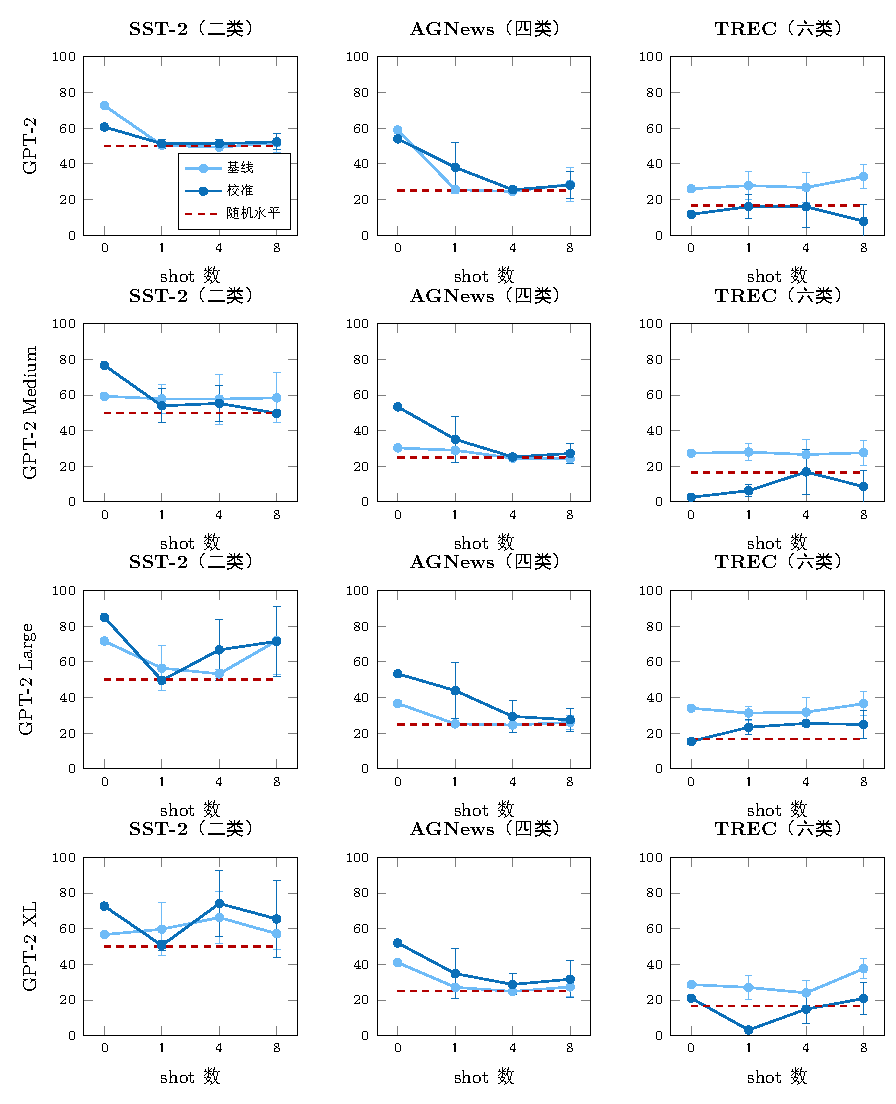
\includegraphics[width=0.88\textwidth]{材料/figures/fig3_fullgrid_acc.pdf}
\caption{全网格准确率（均值$\pm$标准差，5 个训练样例集合）随 shot 数变化：基线 vs 校准，
虚线为随机水平。每个面板 20 个 run（4 shots 配置 $\times$ 5 seeds），共 240 run。}
\label{fig:fullgrid}
\end{figure}

\section{消融实验：内容无关输入的选择（Table 3）}

按论文 Table 3 的设置（1-shot SST-2、0-shot AGNews），对每种内容无关输入选择单独计算
$p_{\mathrm{cf}}$ 并重算校准准确率（每个 run 的逐样本概率复用主实验落盘结果，
单输入 $p_{\mathrm{cf}}$ 为新增前向）；表~\ref{tab:abl} 为 5 seeds 均值，全量 50 条记录见
\texttt{results/cf\_ablation/}。

\begin{table}[h]\centering\small
\begin{tabular}{llcccc}
\toprule
设置 & 模型 & 三者平均 & N/A & [MASK] & 空串 \\
\midrule
\multirow{4}{*}{SST-2 1-shot}
 & gpt2        & 0.5133 & 0.5093 & 0.4887 & 0.4947 \\
 & gpt2-medium & 0.5393 & 0.5340 & 0.4960 & 0.5400 \\
 & gpt2-large  & 0.4960 & 0.4960 & 0.4960 & 0.4960 \\
 & gpt2-xl     & 0.5060 & 0.4960 & 0.5087 & 0.5480 \\
\midrule
\multirow{4}{*}{AGNews 0-shot}
 & gpt2        & 0.5400 & 0.5333 & 0.5533 & 0.5567 \\
 & gpt2-medium & 0.5333 & 0.5333 & 0.5333 & 0.5333 \\
 & gpt2-large  & 0.5333 & 0.5133 & 0.5033 & 0.5233 \\
 & gpt2-xl     & 0.5200 & 0.5233 & 0.5533 & 0.5733 \\
\bottomrule
\end{tabular}
\caption{内容无关输入选择消融（校准准确率，5 seeds 均值，对应论文 Table 3 设置）。}
\label{tab:abl}
\end{table}

\textbf{复现结论：内容无关输入的选择实质性影响结果，且存在多种好选择}（论文 Table 3 的结论）。
最显著处：XL AGNews 0-shot 空串 0.5733 vs 三者平均 0.5200（差 5.3pp）；单输入与三者平均
互有胜负（24 组对比中 8 优 / 6 平 / 10 劣）。8 组配置中 6 组四值互异（2 组完全相同）。
四值完全相同的组（medium AGNews 0-shot 与 large SST-2 1-shot）均为
\textbf{坍缩机制}：校准后全部样本坍缩到同一类，$\arg\max$ 对 $p_{\mathrm{cf}}$ 不敏感——
这本身即"校准可能失效"的边界证据。gpt2 全部 12 个配置的消融也已完成（复用同一管线），
TREC 8-shot 上三者平均 0.0333 vs [MASK] 0.2400，选择差异高达 20.7pp。

\begin{figure}[h]\centering
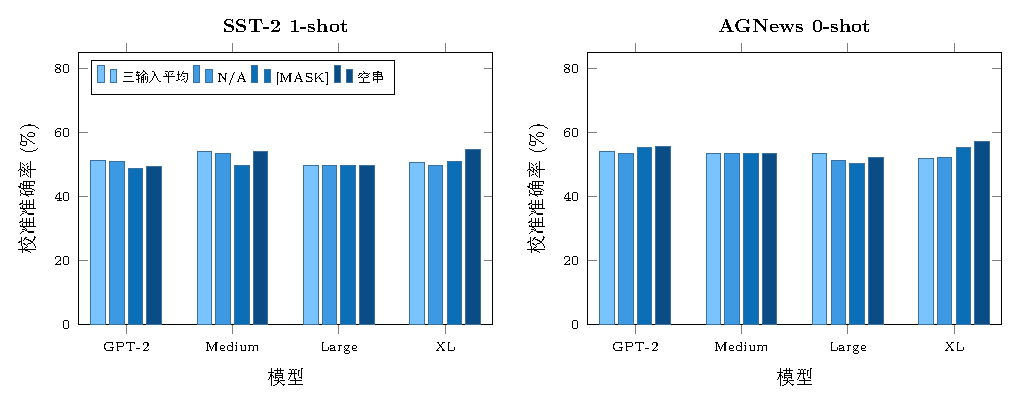
\includegraphics[width=0.98\textwidth]{材料/figures/fig4_table3_ablation.pdf}
\caption{Table 3 消融分组柱状图（左：SST-2 1-shot；右：AGNews 0-shot）。}
\label{fig:abl}
\end{figure}

\section{案例分析}

全部 240 个 run 的逐样本统计：校准翻转预测 48802 例 = \textbf{校准修复 14688}（基线错$\rightarrow$校准对）
+ \textbf{校准破坏 16089}（基线对$\rightarrow$校准错）+ \textbf{双向翻错 18025}（两次预测均非 gold）。
逐例明细（含原文、两套预测、校准前后概率）共 24 例见 \texttt{results/案例分析\_全量.md}，
此处精讲三例（数值均可从逐样本 CSV 复算）：

\textbf{案例 1（校准修复，先验抑制机制）}：gpt2 $\times$ AGNews $\times$ 1-shot（seed 1，
样本 4660）体育新闻（Jim Leyland 教练人事新闻，gold=Sports）。基线 Sports 0.4960 与
Business 0.4986 几乎打平，以 0.26pp 之差错判 Business；校准分数变为 Sports 443.2 vs
Business 9.2，强势翻正——Business 类的先验成分被 $1/p_{\mathrm{cf}}$ 抑制，微弱的真实信号被放大。

\textbf{案例 2（校准破坏，TREC 坍缩机制）}：gpt2-medium $\times$ TREC $\times$ 1-shot（seed 3，
样本 240）``What French province is cognac produced in?''（gold=LOC）。基线六类近乎均匀
（LOC 0.2141 微弱领先，正确）；校准后 ABBR 分数 271.3 一骑绝尘，翻错——ABBR 类的
$p_{\mathrm{cf}}$ 极小导致 $1/p_{\mathrm{cf}}$ 极大，均匀分布上的微小噪声被放大成强坍缩。
这是 TREC 全规模负收益（\S5 结论二）的样本级机制。

\textbf{案例 3（双向翻错）}：gpt2 $\times$ TREC $\times$ 0-shot（样本 272，gold=DESC），
基线判 NUM、校准判 ABBR，两次预测均非 gold。此类占全部翻转的 37\%（18025/48802），
说明坍缩方向与样本真实类别无关，进一步支持"TREC 上校准引入的是与内容无关的偏移"。

\section{结论与讨论}

\textbf{复现成功}：(1) 校准提升平均准确率的主结论在 $\geq$355M 规模、低 shot（0/1）与
SST-2/AGNews 上方向稳定复现（最高 $+$23.0pp）；(2) Table 3"内容无关输入的选择影响结果、
存在多种好选择"完整复现；(3) 先验坍缩与回声机制与原文描述一致。

\textbf{未复现 / 不一致}：(1) TREC 上原文报告校准全面正收益，本组四模型全面负收益
（机制证据：均匀先验下的噪声放大，案例 2）；(2) 降方差声称未复现（26/36 配置升方差）。

\textbf{讨论}：两处不一致的共同背景是本组为缩规模复现（124M--1.5B vs 175B）+ 300 条固定子集
+ 训练集划分与论文表格存在作者自声明的差异。TREC 的负结果方向与原文"校准可能伤害性能"的
警示（原文 \S5 及其 Figure 4 的失败案例分析）一致，可视为该警示在更小规模、
标签先验差距小的任务上的放大呈现。

\textbf{局限与后续}：未复现 GPT-3 API 规格；单一 prompt 格式（附录 B 主格式）；
训练样例排列敏感性（原文 Figure 2/3）未纳入本组范围。后续可对 TREC 做标签词替换
与 $p_{\mathrm{cf}}$ 结构分析以定位不一致来源。

\begin{thebibliography}{9}\small
\bibitem{zhao21} T. Zhao, E. Wallace, S. Feng, D. Klein, S. Singh.
  \emph{Calibrate Before Use: Improving Few-Shot Performance of Language Models}.
  ICML 2021, PMLR 139.
\bibitem{code} T. Zhao. \emph{few-shot-learning}（作者开源代码，Apache 2.0）.
  \texttt{github.com/tonyzhaozh/few-shot-learning}，master 分支（本组参考副本见 \texttt{作者代码/}）.
\end{thebibliography}

\appendix
\section{来源与 AI 辅助声明}
数据来源、许可与 SHA256 见 \texttt{code/data/README.md}；模型权重为 HuggingFace 公开 GPT-2
（hf-mirror.com 获取，版本与校验见 \texttt{code/README.md} \S3.3）；本组代码与作者代码的 9 项
差异逐条声明于 \texttt{code/README.md} \S6。AI 辅助（Claude Code）仅用于工程实现、批量执行、
汇总图件与多代理交叉复核，全部实验在本机 GPU 实际运行，每个数字可溯源到 \texttt{results/}
下具体文件；实验方案、结果判读与结论由本组成员完成。成员分工见 \texttt{contributions.md}。

\end{document}
